\subsection{Inflow Boundary Condition}

\subsubsection{Continuity}
Continuity uses a flux boundary condition with the incoming
mass flow rate based on the user specified values for velocity,
\begin{equation}
  \dot{m}_c = \rho^{spec} u^{spec}_j A_j.
\end{equation}
As this is a vertex-based code, at inflow and Dirichlet wall boundary locations,
the continuity equation uses the specified velocity within the inflow boundary condition
block.

\subsubsection{Momentum, Mixture Fraction, Enthalpy, Species, $k_{sgs}$, k and $\omega$}
These degree-of-freedoms (DOFs) each use a Dirichlet value with the specified user value.
For all Dirichlet values, the row is zeroed with a unity placed
on the diagonal. The residual is zeroed and set to the difference
between the current value and user specified value.

\subsection{Wall Boundary Conditions}

\subsubsection{Continuity}
Continuity uses a no-op.

\subsubsection{Momentum}
When resolving the boundary layer, Momentum again uses a no-slip 
Dirichlet condition., e.g., $u_i = 0$. 

In the case of a wall model, a classic wall function is applied.
The wall shear stress enters the discretization of the momentum equations 
by the term
%
\begin{equation}
        \int \tau_{ij} n_j dS = -{F_w}_i .
 \label{wall_shear1}
\end{equation}
%
Wall functions are used to prescribe the value of the wall shear 
stress rather than resolving the boundary layer within the near-wall 
domain. The fundamental momentum law of the wall formulation, assuming 
fully-developed turbulent flow near a no-slip wall, can be written as,
%
\begin{equation}
u^+ = {u_{\|} \over u_{\tau}} 
    = { 1 \over \kappa } \ln \left(Ey^+\right) ,
\label{law_wall}
\end{equation}
%
where $u^+$ is defined by the the near-wall parallel velocity, $u_{\|}$, normalized 
by the wall friction velocity, $u_{\tau}$. The wall friction velocity is
related to the turbulent kinetic energy by,
%
\begin{equation} 
        u_{\tau} = C_\mu^{1/4} k^{1/2}.
\label{utau}
\end{equation}
%
by assuming that the production and dissipation of turbulence is in local 
equilibrium.  The wall friction velocity is also computed given the density and wall shear stress,
\begin{equation} 
        u_\tau = (\frac{\tau_w} {\rho})^{0.5}.
\end{equation}


The normalized perpendicular distance from the point in question to the wall, $y^+$, is defined as
the following:
%
\begin{equation} 
        y^+ = {{ \rho Y_p} \over {\mu }}\left(\tau_w \over \rho \right)^{1/2} 
            = {{ \rho Y_p u_{\tau}} \over {\mu }}.
\label{yplus}
\end{equation}
%
The classical law of the wall is as follows:
%
\begin{equation}
       u^+ = \frac{1}{\kappa} \ln(y^+) + C,
\label{lawOfWall1}
\end{equation}
%
where $\kappa$ is the von Karman constant and $C$ is the dimensionless 
integration constant that varies based on authorship and surface roughness. 
The above expression can be re-written as,
%
\begin{equation}
       u^+ = \frac{1}{\kappa} \ln(y^+) + \frac{1}{\kappa} \ln(\exp(\kappa C)),
\label{lawOfWall2}
\end{equation}
%
or simplified to the following expression:
%
\begin{align}
       u^+ &= \frac{1}{\kappa} \left(\ln(y^+) + \ln(\exp(\kappa C))\right) \\
           &= \frac{1}{\kappa} \ln(E y^+).
\label{lawOfWall3}
\end{align}
%
In the above equation, $E$, is referred to in the text as the dimensionless wall 
roughness parameter and is described by,
%
\begin{equation}
       E = \exp(\kappa C).
\label{ElogParam}
\end{equation}
%
In Nalu, $\kappa$ is set to the value of 0.42 while the 
value of $E$ is set to 9.8 for smooth walls\footnote{White 
suggests values of $\kappa=0.41$ and $E=7.768$.}. 
The viscous sublayer is assumed to extend to a value of $y^+$ = 11.63.

The wall shear stress, $\tau_w$, can be expressed as,
%
\begin{equation} 
        \tau_w = \rho u_\tau^2 = \rho u_\tau {{u_\|} \over {u^+}}
               = { {\rho \kappa u_{\tau}}  \over {\ln \left(Ey^+\right) } }u_\|
               = \lambda_w u_\| ,
\label{wall_shear_trb}
\end{equation}
%
where $\lambda_w$ is simply the grouping of the factors from the law of the wall.
For values of $y^+$ less than 11.63, the wall shear stress is given by,
%
\begin{equation}
        \tau_w =  \mu {u_\| \over Y_p} .
\label{wall_shear_lam}
\end{equation}
%
The force imparted by the wall, for the $i_{th}$ component of velocity,
can be written as,
%
\begin{equation}
        F_{w,i}= -\lambda_w A_w u_{i\|} ,
\label{wall_force_1}
\end{equation}
%
where $A_w$ is the total area over which the shear stress acts.

The use of a general, non-orthogonal mesh adds a slight complexity to 
specifying the force imparted on the fluid by the wall.
As shown in Equation~\ref{wall_force_1}, the velocity component parallel to 
the wall must be determined. Use of the unit normal vector, $n_j$, 
provides an easy way to determine the parallel velocity component by the 
following standard vector projection:
%
\begin{equation}
        \Pi_{ij} = \left [ \delta_{ij} - n_i n_j \right].
\label{proj_oper}
\end{equation}
%
Carrying out the projection of a general velocity,
which is not necessarily parallel to the wall, yields the velocity vector 
parallel to the wall,
%
\begin{equation}
        u_{i\|} = \Pi_{ij} {u}_j = u_i\left(1-{n_i}^2\right)
        -\sum_{j=1;j\neq j}^{n} u_j n_i n_j.
\label{proj_operU}
\end{equation}
%
Note that the component that acts on the particular $i^{th}$ component of 
velocity,
%
\begin{equation}
        -\lambda_w A_w \left(1-n_i n_i\right) u_{i\|} ,
\label{implicit_shear}
\end{equation}
%
provides a form that can be potentially treated implicitly; i.e., in a way to 
augment the diagonal dominance of the central coefficient of the $i^{th}$ 
component of velocity. The use of residual form adds a slight complexity to
this implicit formulation only in that appropriate right-hand-side source terms
must be added.

\subsubsection{Mixture Fraction}
If a value is specified for each quantity within the wall boundary condition block, a Dirichlet condition
is applied. If no values are specified, a zero flux condition is applied.

\subsubsection{Enthalpy}
If the temperature is specified within the wall boundary condition block, a Dirichlet condition
is always specified. Wall functions for enthalpy transport have not yet been implemented. 

The simulation tool supports multi-physics coupling via conjugate heat transfer and radiative heat transfer.
Coupling parameters required for the thermal boundary condition are post processed by the fluids or PMR Realm.
For conjugate and radiative coupling, the thermal solve provides the surface temperature. From the surface temperature, 
a wall enthalpy is computed and used.

\subsubsection{Thermal Heat Conduction}
If a temperature is specified in the wall block, and the surface is not an interface condition, then a Dirichlet
approach is used. If conjugate heat transfer is included, then
the boundary condition applied is as follows,

\begin{equation}
     -\kappa \frac{\partial T} {\partial x_j} n_j dS = h(T-T^o)dS,
\end{equation}
where $h$ is the heat transfer coefficient and $T^o$ is the reference
temperature. The details of how these quantities are computed are currently omitted
in this manual. In general, the quantities are post processed from the fluids temperature field. A surface-based
gradient is computed on the boundary face. Nodes on the face augment a heat transfer coefficient field while
nodes off the face contribute to a reference temperature. 

For radiative heat transfer, the boundary condition 
applied is as follows:
\begin{equation}
     -\kappa \frac{\partial T} {\partial x_j} n_j dS = \epsilon (\sigma T^4 - H) dS,
\end{equation}
where $H$ is again the irradiation provided by the RTE solve.

If no temperature is specified or an adiabatic line command is used, a zero flux condition is applied.

\subsubsection{Species}
If a value is specified for each quantity within the wall boundary condition block, a Dirichlet condition
is applied. If no values are specified, a zero flux condition is applied.

\subsection{Atmospheric Boundary Layer Surface Conditions}
\subsubsection{Monin-Obukhov Theory}
Consider atmospheric flow over a flat but non-smooth surface; the
coordinate system convention is that flow is along the $x$-axis, while
the $z$-axis is oriented normal to the surface.  The surface layer is
the relatively thin layer near the surface where strong wind and
temperature gradients exist.  Turbulence within this layer can be
generated through mechanisms of both shear and thermal convection; the
relative contributions of these two mechanisms is determined by the
stability state of the atmosphere.  The stability state is
characterized by the Monin-Obukhov length:
\begin{equation}
 L = - \frac{u_\tau^3 \theta_{ref}}{\kappa g (\overline{w^\prime
     \theta^\prime})_s};
\end{equation}
$u_\tau$ is the friction velocity, defined as the
square root of the magnitude of the Reynolds shear stress at
the surface, or
\begin{equation}
 u_\tau = \left( \overline{w^\prime u^\prime}^2 + \overline{w^\prime
   u^\prime}^2 \right)^{1/4} = \sqrt{\frac{\tau_s}{\rho_s}}
\end{equation}
$\theta_{ref}$ is a reference (virtual potential) temperature associated with the air
within the surface layer; for example, the average temperature within
the surface layer.  $\kappa \approx 0.41$ is the von Karman constant,
and $g$ is the acceleration of gravity.  $\overline{w^\prime
     \theta^\prime}_s$ is the surface turbulent temperature flux.  Both the
turbulent shear stress and turbulent temperature flux are approximately
constant within the surface layer.

Applying a gradient diffusion model for the turbulent temperature flux leads to:
\begin{equation}
 \overline{w^\prime \theta^\prime}_s = -k_T \pd{\theta}{z}
\end{equation}.
The sign of $L$ is then connected to the sign of the temperature
gradient within the surface layer.  Three regimes are delineated:
\begin{itemize}
  \item $\frac{1}{L} > 0, \quad \pd{\theta}{z} > 0$~~~stable
    stratification
  \item $\frac{1}{L} = 0, \quad \pd{\theta}{z} = 0$~~~neutral
    stratification
  \item $\frac{1}{L} < 0, \quad \pd{\theta}{z} < 0$~~~unstable stratification
\end{itemize}

Monin-Obukhov theory postulates the following similarity laws for mean
velocity parallel to the surface and temperature,
\begin{equation} \label{dudz}
\frac{\kappa z}{u_\tau}\pd{\overline{u}_{||}}{z} =
\phi_m\left(\frac{z}{L}\right),
\end{equation}
\begin{equation} \label{dTdz}
\frac{\kappa z u_\tau}{\overline{w^\prime \theta^\prime}_s}
\pd{\overline{\theta}}{z} = \phi_h\left(\frac{z}{L}\right),
\end{equation}
where the forms of the non-dimensional functions $\phi_m$ and $\phi_h$ are determined
from empirical observations. Analytical functions have been fit to the
data; these are not given here, rather, we present the integrated form
of (\ref{dudz}) and (\ref{dTdz}), since these are the forms required
by the code implementation.

For neutral stratification, $\phi_m = 1$ and we recover the
logarithmic profile for a ``fully rough'' surface,
\begin{equation} \label{vel_neutral}
\overline{u}_{||}(z) = \frac{u_\tau}{\kappa}\ln\frac{z}{z_0},
\end{equation}
where $z_0$ is the characteristic roughness height.  Note that viscous
scaling involving surface viscosity and density properties is not
required with this form of the logarithmic profile, since the
roughness height is large enough to eliminate the presence of a
laminar sublayer and buffer layer.

For stable stratification, the surface layer profiles take the form
\begin{equation} \label{vel_stable}
 \overline{u}_{||}(z) = \frac{u_\tau}{\kappa}\left(\ln\frac{z}{z_0} +
 \gamma_m\frac{z}{L}\right)
\end{equation}
\begin{equation}  \label{temp_stable}
\overline{\theta}(z) = \overline{\theta}(z_0) +
\frac{\theta_*}{\kappa} \left(\alpha_h\ln\frac{z}{z_0} +
\gamma_h\frac{z}{L}\right)
\end{equation}
$\theta_*$ is calculated from the temperature flux and friction velocity as
$\theta_* = -\frac{\overline{w^\prime \theta^\prime}_s}{u_\tau}$, and
$\gamma_m$, $\alpha_h$, and $\gamma_h$ are constants specified below.

For unstable stratification, the surface layer profiles take the form
\begin{equation} \label{vel_unstable}
  \overline{u}_{||}(z) = \frac{u_\tau}{\kappa}\left(\ln\frac{z}{z_0} -
  \psi_m\left(\frac{z}{L}\right)\right)
\end{equation}
\begin{equation} \label{temp_unstable}
  \overline{\theta}(z) = \overline{\theta}(z_0) +
  \alpha_h\frac{\theta_*}{\kappa}\left(\ln\frac{z}{z_0} -
  \psi_h\left(\frac{z}{L}\right)\right)
\end{equation}
where
\begin{equation} \label{psi_m}
 \psi_m\left(\frac{z}{L}\right) = 2\ln\frac{1 + x}{2} + \ln\frac{1 + x^2}{2} - 2\tan^{-1}x +
 \frac{\pi}{2}, \quad x = \left(1 - \beta_m\frac{z}{L}\right)^{1/4},
\end{equation}
\begin{equation} \label{psi_h}
 \psi_h\left(\frac{z}{L}\right) = \ln\frac{1 + y}{2}, \quad y = \left(1 -
 \beta_h\frac{z}{L}\right)^{1/2}.
\end{equation}

The constants used in (\ref{vel_stable}) -- (\ref{psi_h}) are \cite{Dyer:74}
\begin{equation}
  \kappa = 0.41,~~\alpha_h =
  1,~~\beta_m=16,~~\beta_h=16,~~\gamma_m=5.0,~~\gamma_h=5.0.
\end{equation}

\subsubsection{ABL Wall Function}
The equations from the preceeding section can be used to formulate a
wall function boundary condition for simulation of atmospheric
boundary layers.  The user-specified inputs to this boundary condition
are: roughness length, $z_0$, and surface heat flux, $q_s =
\rho C_p \overline{w^\prime \theta^\prime})_s$.  The surface layer profile
model is evaluated for each surface boundary flux integration point;
the wall-normal distance of the ``first point off the wall'' is taken
to be one fourth of the length of the nearest edge intersecting the
boundary face.  The boundary condition is specified weakly through the
imposition of a surface shear stress and surface heat flux.

The procedure for applying the boundary condition is as follows.
\begin{enumerate}
\item Determine the stratification state of the boundary layer by
  calculating the sign of the Monin-Obukhov length scale.
\item Solve the appropriate profile equation, either
  (\ref{vel_neutral}), (\ref{vel_stable}), or (\ref{vel_unstable}),
  for the friction velocity $u_\tau$.  For the neutral case, $u*$ can be
  solved for directly.  For the stable and unstable cases, $u*$ must
  be solved for iteratively because $L$ appears in these equations and
  $L$ depends on $u_\tau$.
\item The surface shear stress is calculated as $\tau_s = \rho_s u_\tau^2$.
  For calculating left-hand-side Jacobian entries, the form $\tau_s =
  \lambda_s u_{||}$ is useful. This form can be found by algebraic
  manipulation of the relevant velocity profile equation.
\item The user specified surface heat flux is applied to the enthalpy
  equation.  Evaluation of surface temperature is not required for
  the boundary condition specification.  However, if surface
  temperature is required for evaluation of other quantities within
  the code, the appropriate surface layer temperature profile should
  be used, either (\ref{temp_stable}) or (\ref{temp_unstable}).
\end{enumerate}

\subsection{Turbulent Kinetic Energy, $k_{sgs}$ LES model}
When the boundary layer is assumed to be resolved, the natural boundary condition is a Dirichlet value of zero, 
$k_{sgs} = 0$. 

When the wall model is used, a standard wall function approach is used with the assumption of equal production and
dissipation.

The turbulent kinetic energy production term is consistent with the law of the wall formulation and can be expressed as,
%
\begin{equation}
        {P_k}_w = \tau_w {{\partial u_{\|}} \over {\partial y}}.
\label{wall_pk_1}
\end{equation}
%
The parallel velocity, $u_{\|}$, can be related to the wall shear stress by,
%
\begin{equation}
        \tau_w {u^+ \over y^+ } = \mu {u_{\|} \over Y_p }.
\label{tauwall_uplus}
\end{equation}
%
Taking the derivative of both sides of Equation~\ref{tauwall_uplus}, and
substituting this relationship into Equation~\ref{wall_pk_1} yields,
%
\begin{equation} 
        {P_k}_w = {\tau_w^2 \over \mu} {{\partial u^+} \over {\partial y^+}}.
\label{wall_pk_2}
\end{equation}
%
Applying the derivative of the law of the wall formulation, Equation~\ref{law_wall},
provides the functional form of ${\partial u^+ / \partial y^+}$,
%
\begin{equation} 
        {\partial u^+ \over \partial y^+}
      = {\partial \over \partial y^+}
       \left[{ 1 \over \kappa } \ln \left(Ey^+\right) \right]
      = {1 \over \kappa y^+}.
\label{dlaw_wall}
\end{equation}
%
Substituting Equation~\ref{dlaw_wall} within Equation~\ref{wall_pk_2} yields
a commonly used form of the near wall production term,
%
\begin{equation}
        {P_k}_w = {{\tau_w}^2 \over \rho\kappa u_{\tau} Y_p}.
\label{wall_pk_3}
\end{equation}
%
Assuming local equilibrium, $P_k = \rho\epsilon$, and using
Equation~\ref{wall_pk_3} and Equation~\ref{utau} provides the form 
of wall shear stress is given by,
%
\begin{equation}
        \tau_w = \rho C_\mu^{1/2} k.
\label{wall_tauw_equil}
\end{equation}
%
Under the above assumptions, the near wall value for turbulent kinetic 
energy, in the absence of convection, diffusion, or accumulation is given by,
%
\begin{equation}
   k = {{u_\tau^2} \over {C_\mu^{1/2}}}.
\label{wall_tke}
\end{equation}

This expression for turbulent kinetic energy is evaluated at the boundary faces of the
exposed wall boundaries and is area-assembled to the nodal value for use in a Dirichlet condition.

\subsubsection{Turbulent Kinetic Energy and Specific Dissipation SST Low Reynolds Number Boundary conditions}

For the turbulent kinetic energy equation, the wall boundary conditions follow that described for 
the $k_{sgs}$ model, i.e., $k=0$.

A Dirichlet condition is also used on $\omega$.  For this boundary condition, the $\omega$ equation depends only on the near-wall 
grid spacing.  The boundary condition is given by,
\begin{equation}
\omega = {6 \nu \over \beta_1 y^{2}},
\end{equation}
which is valid for $y^{+} < 3$. 

\subsubsection{Turbulent Kinetic Energy and Specific Dissipation SST High Reynolds Number Boundary conditions}
The high Reynolds approach uses the law of the wall assumption and also follows the description 
provided in the wall modeling section with only a slight modification in constant syntax,

\begin{equation}
k = {u_{\tau}^{2} \over \sqrt{\beta^*}}.
\label{wallModelTke}
\end{equation}
% 
In the case of $\omega$, an analytic expression is known in the log layer:
\begin{equation}
\omega = {u_{\tau} \over \sqrt{\beta^*} \kappa y},
\end{equation}
which is independent of $k$.  Because all these expressions require $y$ to be in the log layer, 
they should absolutely not be used unless it can be guaranteed that $y^{+} > 10$, and $y^{+} > 25$ is preferable.
%
Automatic blending is not currently supported.

\subsubsection{Solid Stress}
The boundary conditions applied are either force provided by a static pressure, 

\begin{equation}
 F^n_i = \int \bar{P} n_i dS,
\label{displacement}
\end{equation}
%
or a Dirichlet condition, i.e., $u_i = u^{spec}_i$, on the displacement field. Above, $F^n_i$ is the force for
component $i$ due to a prescribed [static] pressure. 

\subsubsection{Intensity}
The boundary condition for each intensity assumes a grey, diffuse surface as, 
\begin{equation}
  I\left(s\right) = {1 \over \pi} \left[ \tau \sigma T_\infty^4 
                  + \epsilon \sigma T_w^4
                  + \left(1 - \epsilon - \tau \right) K \right].
\label{intBc}
\end{equation}

\subsection{Open Boundary Condition}
Open boundary conditions require far more care. In general,
open bcs are assembled by iterating faces and the boundary integration
points on the exposed face. The parent element is also required
since oftentimes gradients are used (for momentum). For an open boundary condition
the flow can either leave or enter the domain depending on what the computed mass
flow rate at the exposed boundary integration point is.

\subsubsection{Continuity}
For continuity, the boundary mass flow rate must also be computed. This value is stored and used
for the other equations that require advection. The same formula is used for the pressure-stabilized 
mass flow rate. However, the local pressure gradient
for each boundary contribution is based on the difference between the interior integration
point and the user-specified pressure which takes on the boundary value. The interior integration 
point is determined by linear interpolation. For CVFEM, full elemental averaging is used while in EBVC discretization,
the midpoint value between the nearest node and opposing node to the boundary integration point is used. In both
discretization approaches, non-orthogonal corrections are required. This procedure has been very important for 
stability for CVFEM tet-based meshes where a natural non-orthogonality exists between the boundary and
interior integration point.

\subsubsection{Momentum}
For momentum, the normal component of the stress is subtracted out we subtract out the normal component of the stress. The normal stress
component for component i can be written as $F_k n_k n_i$. The tangential 
component for component i is simply, $F_i - F_k n_k n_i$. As an example, the tangential
viscous stress for component x is,

\begin{equation}
  F^T_x = F_x - (F_x n_x + F_y n_y ) n_x,
\end{equation}
which can be written in general component form as,
\begin{equation}
  F^T_i = F_i(1-n_i n_i) - \sum_{i!=j} F_j n_i n_j.
\end{equation}

Finally, the normal stress contribution is applied based on the user specified pressure,
\begin{equation}
  F^N_i = P^{Spec} A_i.
\end{equation}

For CVFEM, the face gradient operators are used for the thermal stress terms. For EBVC discretization, 
from the boundary integration
point, the nearest node (the ``Right'' state) is used as well as the opposing node
(the ``Left'' state). The nearest node and opposing node are used to compute
gradients required for any derivatives. This equation follows the standard
gradient description in the diffusion section with non-orthogonal corrections used.
In this formulation, the area vector is taken to be the exposed area vector. 
Non-orthogonal terms are noted when the area vector and edge vector are not aligned.

For advection, If the flow is leaving the domain, we simply advect the nearest nodal value
to the boundary integration point. If the flow is coming into the domain,
we simply confine the flow to be normal to the open boundary integration 
point area vector. The value entrained can be the nearest node
or an upstream velocity value defined by the edge midpoint value. 

\subsubsection{Mixture Fraction, Enthalpy, Species, $k_{sgs}$, k and $\omega$ }
Open boundary conditions assume a zero normal gradient. When flow is entering the domain, the far-field
user supplied value is used. Far field values are used for property evaluations. When flow is leaving the domain, 
the flow is advected out consistent with the
choice of interior advection operator.

\subsection{Symmetry Boundary Condition}

\subsubsection{Continuity, Mixture Fraction, Enthalpy, Species, $k_{sgs}$, k and $\omega$}
Zero diffusion is applied at the symmetry bc.

\subsubsection{Momentum}
A symmetry boundary is one that is described by removal of the tangential stress. Therefore, only
the normal component of the stress is applied:

\begin{equation}
  F^n_x = (F_x n_x + F_y n_y ) n_x,
\end{equation}
which can be written in general component form as,
\begin{equation}
  F^n_i = F_j n_j n_i.
\end{equation}

\subsection{Periodic Boundary Condition}
A parallel multiple-periodic boundary condition is supported. Mappings are created between
master/slave surface node pairs. The node pairs are obtained from a parallel search and are expected
to be unique. The node pairs are used to map the slave global id to that of the master. This allows the linear
system to include matrix rows for only a subset of the overall set of nodes. Moreover, a periodic 
assembly for assembled quantities is managed via: $m+=s$ and $s=m$, where $m$ and $s$ are master/slave nodes, 
respectively. For each parallel assembled quantity, e.g., dual volume, turbulence quantities, etc., this procedure
is used. Periodic boxes and periodic couette and channel flow have been simulated in this code base. Tow forms of
parallel searches exist and are supported (one through the Boost TPL and another through the STK Search module).

\subsection{Contact Boundary Condition}
Parallel sliding mesh algorithm based on extension of Blades,~\cite{Blades:2004}, to the low Mach application 
space. This capability is available in 2D and 3D. It has been designed for use in the EBVC approach, although 
CVFEM can also be used. In this formulation, the exposed  surface is extruded into the opposing block's mesh.
For two dimensional meshes, the edge face (from either a tri or quad mesh) is extruded as a quad mesh
into the opposing block. For three dimensional meshes, the quad face is extruded as a hex element.

Conceptually, the algorithm works as follows: First, the dual mesh is defined by identifying
the ordinal of the exposed surface from its owning element. Mappings between each ordinal and the
extruded element are made to determine how the extruded element is used to close the halo edge area vector,
edge area vector already defined on the exposed side's set of edges and the dual volume at the exposed
side nodes.

In Figure~\ref{quad-halo}, consider that the side that is comprised by node 2 and node 3 represents 
the exposed surface in question. This exposed surface, as defined by the Exodus II standard, is ordinal number two. 
Conceptually, the extruded element is obtained by orientating ordinal one of this element to lie on top of the exposed 
ordinal in question. Data structures are defined that map the exposed set of nodes to the extruded 
nearest node and extruded opposing nodes. Moreover, the mapping of subcontrol area vectors within 
the extruded element are provided.  

In this simple quad example, it is noted that the mappings for all
ordinals for the set of boundary element ordinals is the same. Specifically, the mapping between 
nearest node 2 and 3 for face ordinal 2 for the matching face nodes of the extruded element are 2 and 1. Moreover, the mapping 
between nearest nodel 2 and 3 for face ordinal 2 for the matching opposing face nodes of the extruded
element are 3 and 4. These node mappings, along with the extruded distance allows definition of the nodal coordinates
of the extruded element. The halo edge area vector for face nodes 2 and 3 on ordinal 2 are subcontrol surface 2 and 4 
while the edge on the exposed face maps to subcontrol surface 1 of the extruded element. Finally, the
alignment of the subcontrol surface area vector and ordinal edge set is required. In the case of ordinal 2, as is the
case for all ordinals, the natural edge definition (points from node 2 to node 3) is opposite of the subcontrol
surface area vector definition (the dual area vector at the sub control surface always points from local node low to
local node high, e.g, node 1->2.

\begin{figure}[ht]
\centerline{\includegraphics[width=3.0in]{images/quadel.pdf}}
\vspace{0.1in}
\caption{Quadraleteral mapping}
\label{quad-halo}
\end{figure}

The same procedure is repeated for the extruded hex element, Figure~\ref{hex-halo}.
In this case, each three dimensional quad face on the exposed contact surface is extruded
into a hex element. For the hex case, the common face ordinal 1 is matched with each of the possible
six exposed surfaces on the exposed face. Again, mappings are defined that allow for the 
assembly of dual nodal volume, halo edge area vector, augmentation of the exposed side edge
sub-control surfaces and edge alignment wrt sub-control surface area vectors. For the hex case, the mappings are
not the same for all exposed surfaces.

Finally, the procedure to define the extrusion direction is based on a nodal surface normal direction.
This quantity is defined by looping over all exposed surface faces and assembling the surface normal to the nodes.

After the dual mesh is defined and associated area vector and dual volumes are assembled, the projected
node for the pseudo edge is matched to an owning element in the opposing block. The search is performed using a
parallel search that allows for the intersection of a sphere (the point that is projected) and the set of bounding boxes
that is determined by all possible opposing block elements. Once the owning element for each projected point
is determined, the appropriate flux contributions for each PDE is constructed. The halo point state is determined by linear
interpolation within the owning element given the local isoparametric coordinates determined in the fine search. Here, the 
fine search is the process whereby the set of candidate bounding boxes for each extruded point are tested to see which
is the best candidate. This process provides the final isoparametric coordinate set for each of the extruded exposed surface
face nodes. Finally, matrix contributions are fully provided for the face nodes. This procedure finds that the row for the
exposed node is augmented by the columns of the nodes on the owing opposing element.

For cases in which rotation of one block defines a sliding mesh interface, the above procedure is replicated, e.g., projection,
dual mesh definition, search and matrix graph initialization.
\begin{figure}[ht]
\centerline{\includegraphics[width=3.0in]{images/hex.pdf}}
\vspace{0.1in}
\caption{Hexahedron mapping}
\label{quad-halo}
\end{figure}

\subsection{Non-conformal Boundary Condition}
A surface-based approach based on a DG method has been discussed in the 2010 CTR summer 
proceedings by Domino,~\cite{Domino:2010}. Both the edge- and element-based formulation 
currently exists in the code base using the CVFEM and EBVC approaches. 

Consider two domains, $A$ and $B$, which have a common interface, $\Gamma_{AB}$,
and a set of interfaces not in common, $\Gamma \backslash \Gamma_{AB}$
(see Figure~\ref{domainAB}), and assume that the solution of the 
time-dependent advection/diffusion equation is to be solved in both domains. 
Each domain has a set of outwardly pointing normals. In this cartoon, the interface 
is well resolved, although in practice this may not be the case. 


\begin{figure} 
  \centerline{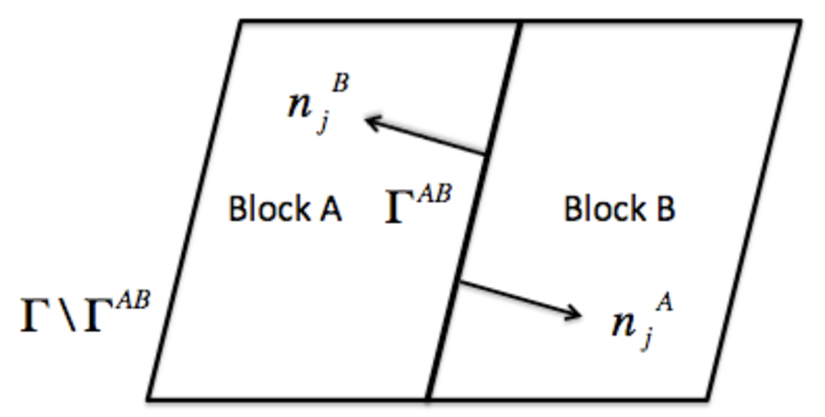
\includegraphics[height=1.5in]{images/twoBlockDiag.pdf}} 
 \caption{Two-block example with one common surface, $\Gamma_{AB}$.} 
 \label{domainAB} 
\end{figure}    

An interior penalty approach is constructed at each integration point at the 
exposed surface set. The numerical flux for a general scalar $\phi$ is constructed at the 
current integration point which is based on the current ($A$) and opposing ($B$) elemental 
contributions,

\begin{equation} 
        \int \hat Q^A dS = \int [\frac{(q_j^A n_j^A + q_j^B n_j^B)}{2}
				+ \lambda^A ( \phi^A - \phi^B) ]dS^A
        				+ \dot{m}^A \frac{(\phi^A + \phi^B)}{2},
\label{numericalFluxA}
\end{equation}
where $q_j^A$ and $q_j^B$ are the diffusive and convective fluxes computed using the current 
and opposing elements. The penalty coefficient $\lambda$ contains both advective and diffusive 
contributions averaged over the two elements. Above, the convection term is Galerkin approach,
however, upwinding has been implemented. Note that the lack of averaging the mass flow rate, 
$\dot{m}^A$ is somewhat arbitrary. The exact form of the mass flow rate is shown below and includes
full pressure stabilization terms.

Since this algorithm is a dual pass approach, a numerical flux can be written for the integration point on block $B$,

\begin{equation} 
        \int \hat Q^B dS = \int [\frac{(q_j^B n_j^B + q_j^A n_j^A)}{2} 
				+ \lambda^B ( \phi^B - \phi^A) ]dS^B
				+ \dot{m}^B \frac{(\phi^B + \phi^A)}{2}.
\label{numericalFluxB}
\end{equation}
Note that in each case, normals are outward facing. For low-order meshes with curved surface, faceting will occur.
In this case, the outward facing normals may not be (sign)-unity factors of each other. In this case, it
may be adventageous to define the opposing outward normal as, $n_j^B = -n_j^A$. 

Average fluxes are computed based on the current and opposing integration point locations. The 
appropriate DG terms are assembled as boundary conditions first with block $A$ integration 
points as $current$ (integrations points for block B are $opposing$) and then with block $B$ 
integration points as $current$ (surfaces for block A are, therefore, $opposing$). Figure~\ref{nonConformal} 
graphically demonstrates the procedure in which integration point values of the flux and penalty 
term are computed on the block $A$ surface and at the projected location of block $B$. 

\begin{figure}
\centering
  {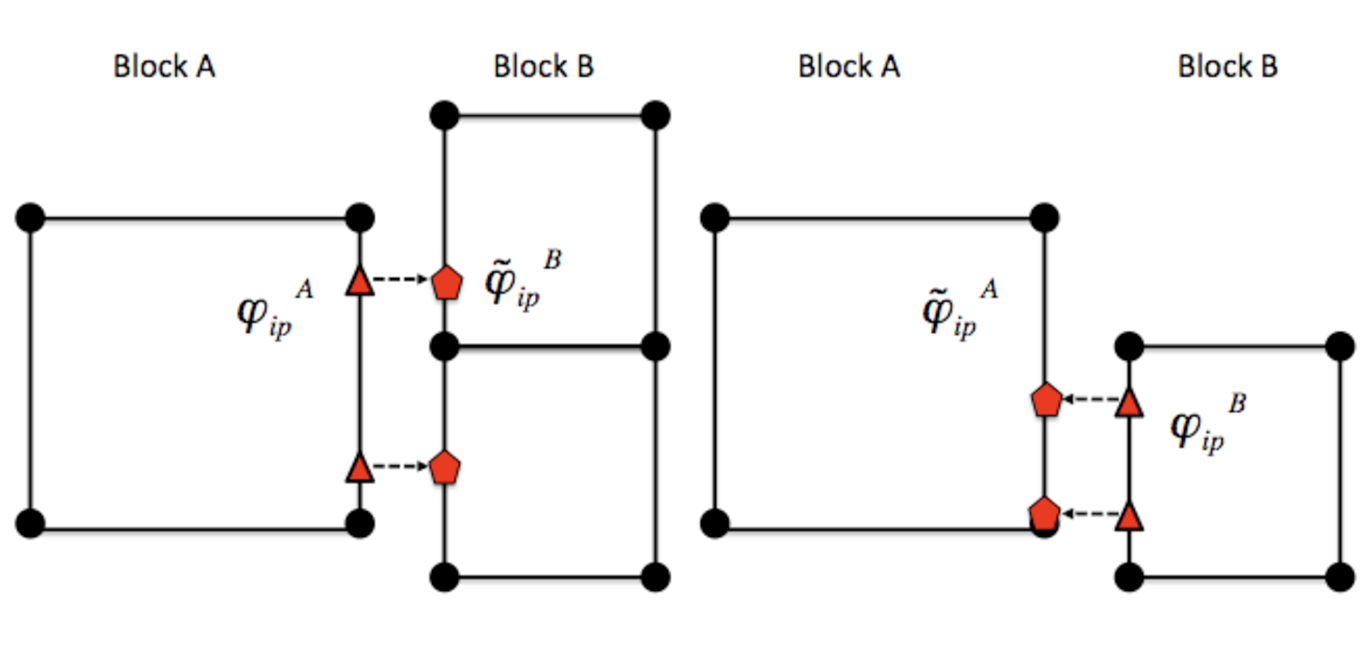
\includegraphics[height=1.5in]{images/contactSearchAndEval.pdf}}
  \vspace{0.25in}
  \caption{Description of the numerical flux calculation for the DG algorithm. The 
    value of fluxes and penalty values on the current block ($A$) and the opposing block ($B$) are used 
    for the calculation of numerical fluxes. $\tilde \varphi$ represents the projected value.}
  \label{nonConformal}
\end{figure}

A parallel search is conducted to project the current integration point location to the opposing element exposed face. 
The search, therefore, provides the isoparametric coordinates on the opposing element. Elemental shape functions 
and shape function derivatives are used to construct the numerical flux for both the edge- and element-based 
scheme. The location of the Gauss points on the current element are either the Gauss Labatto or Gauss Legendre 
locations (input file specification). For each equation (momentum, continuity, enthalpy, etc.) the numerical 
flux is computed at each exposed non-conformal surface.

The value of the penalty parameter, $\lambda$ contains advection and diffusion contributions. The current 
formulation defines this quantity as follows (here shown for current side $A$):

\begin{equation} 
        \lambda^A = \frac{(\Gamma^A / L^A + \Gamma^B / L^B )}{2} + |\dot{m}^A|,
\label{lamdbaA}
\end{equation}
where $\Gamma^k$ is the diffusive flux coefficient evaluated at current and opposing element location, respectively, 
and $L^k$ is an elemental length scale normal to the surface (again for current and opposing locations, $A$ and $B$). 
Again, the form of the penalty term is somewhat arbitrary in that the advection mass flow rate could have been upwinded 
or blended.

As noted, for most equations other than continuity and heat condition, the numerical flux includes advection and 
diffusion contributions. The diffusive contribution is easily provided using elemental shape function derivatives 
at the current and opposing surface. 

Above, special care is taken for the value of the mass flow rate at the non-conformal interface. Also,
note that the above written form does not upwind the advective flux, although the code allows for an upwinded 
approach. In general, the advective term contains contributions from both elements identified at the interface, 
specifically,

\begin{equation} 
        \dot {m}^A = \int [\frac{(\rho u_j^A + \tau G_j^A p -\tau \frac{\partial p^A}{\partial x_j}) 
        				       + (\rho u_j^B+ \tau G_j^B p -\tau \frac{\partial p^A}{\partial x_j})}{2}
				       + \lambda^A ( p^A - p^B)] dS^A.
\label{mdotA}
\end{equation}
The penalty coefficient for the mass flow rate at the non-conformal boundary points is again a function of the 
blended inverse length scale at the current and opposing element surface location. The form of the mass flow 
rate above provides the continuity contribution and the form of the mass flow rate used in the scalar non-conformal
flux contribution.

The full connectivity for element integration and opposing elements is within the linear 
system. As such, for sliding mesh configurations, the linear system connectivity graph changes each time step. Recent prototyping of 
the dG-based and the overset scheme has allowed this method to be used across both disparate low-order 
topologies (see Figure~\ref{dgMixMatch}).

\begin{figure}[h!tp]
\centering
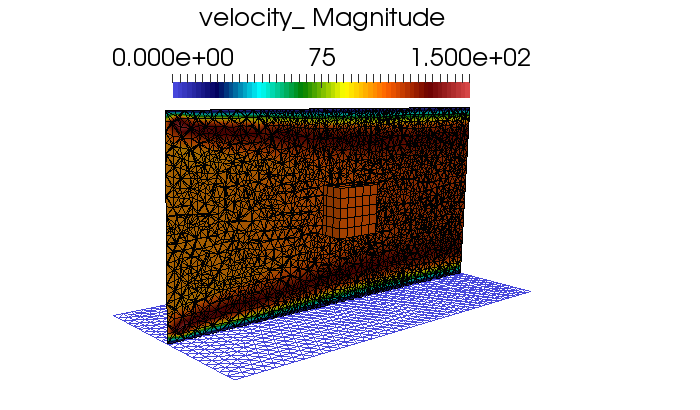
\includegraphics[clip,width=0.4\textwidth]{images/dgHex8Tet4Duct.png}
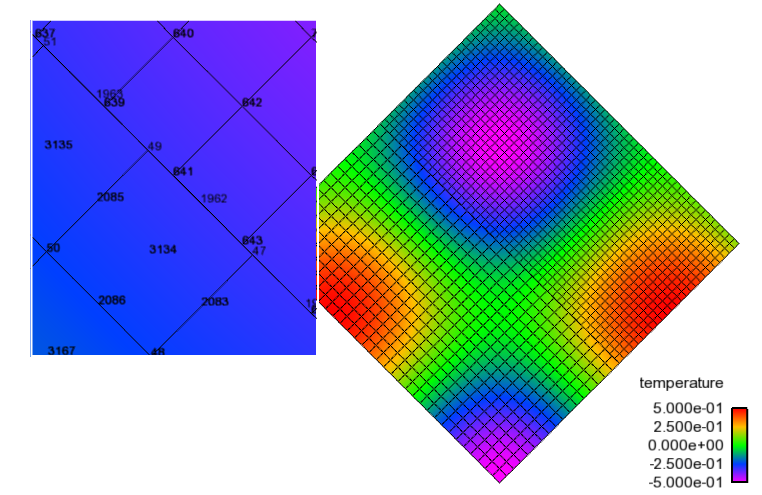
\includegraphics[clip,width=0.4\textwidth]{images/dgQuad4Quad9MMS.png}
\caption{Discontinuous Galerkin non-conformal interface mixed topology (left, hex8/tet4) and a low-order and high-order block interface 
(P=1 quad4 and P=2 quad9) for a MMS temperature solution (right). In the MMS image, the inset image is a close-up of the nodal 
Ids near the interface that highlights the quad4 and quad9 interface.}
\label{dgMixMatch}
\end{figure}
